\documentclass[11pt,letterpaper]{article}
\usepackage[utf8]{inputenc}
\usepackage[spanish]{babel}\decimalpoint
\usepackage{amsmath}
\usepackage{amsfonts}
\usepackage{amssymb}
\usepackage{physics}
\usepackage{hyperref}
\usepackage[left=2cm,right=2cm,top=2cm,bottom=2cm]{geometry}


\usepackage{graphicx}
\graphicspath{{img_tarea-04/}}
\usepackage{subfig}


\usepackage[draft,inline,nomargin]{fixme} \fxsetup{theme=color}
\definecolor{jacolor}{RGB}{200,40,0} \FXRegisterAuthor{ja}{aja}{\color{jacolor}JA}

\newcommand{\mcM}{\mathcal{M}}

\renewcommand{\labelenumii}{\arabic{enumi}.\arabic{enumii}}
\renewcommand{\labelenumiii}{\arabic{enumi}.\arabic{enumii}.\arabic{enumiii}}
\renewcommand{\labelenumiv}{\arabic{enumi}.\arabic{enumii}.\arabic{enumiii}.\arabic{enumiv}}

%%%%% Author
\author{José Alfredo de León}

%%%% Title 
\title{Tarea 4\\
\large{Métodos de Simulación Computacional para Sistemas Cuánticos - 2022-2}}


\begin{document}
\date{28 de febrero de 2022}
\maketitle

\section{Objetivos}
\subsection{Objetivo general}
Resolver numéricamente la diagonalización del Hamiltoniano del modelo de Bose-Hubbard.

\subsection{Objetivos específicos}
\begin{enumerate}
\item Investigar algunas cantidades que permitan estudiar la física
del modelo de Bose-Hubbard, como la fase de condensado, los potenciales 
químicos, el gap de energía, el valor esperado de la energía cinética 
y las fluctuaciones en el número de ocupación.
\item Implementar en Mathematica la construcción del Hamiltoniano 
del modelo de Bose-Hubbard para $N$ partículas y $M$ sitios. 
\item Implementar en Mathematica el código necesario para implementar
el estudio numérico de las cantidades físicas de interés.
\item Mejorar, respecto a las tareas anteriores, la presentación
de las gráficas. 
\end{enumerate}

\section{Marco teórico}
Transisiones cuánticas de fase en gases de Bose en redes ópticas 
están asociadas con correlaciones complejas del estado de muchas partículas.
El modelo de Bose-Hubbard es un modelo teórico que puede describir 
este tipo de correlaciones dominantes. El modelo fue inicialmente 
introducido para estudiar líquidos ${}^4$He en medios porosos y
superconductores granulares, pero también se ha aplicado para 
gases atómicos ultrafríos en redes ópticas \cite{}.

La suposición del modelo de Bose-Hubbard es que los pozos en la red son
suficientemente profundos para que el estado del sistema sea descrito
utilizado la base de funciones de onda de partículas individuales
localizadas en los sitios individuales de la red. 

Los estados del sistema de bosones pueden escribirse utilizando
la representación de los números de ocupación. Supongamos que el 
sistema consiste de $N$ bosones en una red compuesta por $M$ sitios.
Ahora introducimos el conjunto de números de ocupación $\{ n_1,\ldots,n_M\}$,
donde cada $n_i$ especifica el número de bosones en el sitio $i$.
El conjunto de los estados de Fock $\ket{n_1,\ldots,n_M}$ para todas
las posibles composiciones de los números de ocupación bajo la 
restricción $\sum_Mn_M=N$ forman una base completa para el espacio de
estados en el modelo de Bose-Hubbard.

Escribimos al Hamiltoniano del modelo de Bose-Hubbard en su forma de 
segunda cuantización como
\begin{align}\label{eq:H:BoseHubbard}
H=-t\sum_{\langle i,j\rangle}\big(a^{\dagger}_{i}a_j+H.C.\big)+
\frac{U}{2}\sum_{i=1}^Mn_i\qty(n_i-1),
\end{align}
donde $a_i$ ($a_i^{\dagger}$) es el operador de aniquilación (creación)
y $n_i$ el operador de número de ocupación. El símbolo $\langle i,j\rangle$
significa índices de sitios adyacentes. El primer término del 
Hamiltoniano en \eqref{eq:H:BoseHubbard} es el término cinético 
que describe el tunelaje entre sitios de los próximos vecinos caracterizado por 
el parámetro $t$. Para este trabajo \textbf{utilizaremos condiciones 
periódicas}. El segundo término describe la interacción de dos cuerpos
en un mismo sitio caracterizada por un parámetro de interacción $U$.

En este trabajo consideraremos las proporciones $t/U$ y $U/t$ para explorar
diferentes regiones del diagrama de fase a temperatura cero del sistema.

Una cantidad de central interés es la matriz de densidad de una partícula
individual (SPDM por sus siglas en inglés ``\textit{Single-particle
density matrix}'') del estado fundamental del sistema total. Esta
matriz de densidad reducida se define como
\begin{align}\label{eq:SPDM}
\rho^(1)_{ij}=\matrixel{\psi_G}{a_i^{\dagger}a_j}{\psi_G},
\end{align}
donde $\ket{\psi_G}$ es el estado fundamental del Hamiltoniano 
\eqref{eq:H:BoseHubbard}.
De acuerdo con el criterio de Penrose-Onsager un condensado está 
presente si y sólo si el eigenvalor más grande $\lambda^*$ de la matriz de densidad 
de una partícula individual \eqref{eq:SPDM} es macroscópico, lo que
significa que el factor de condensado, definido como
\begin{align}\label{eq:fc}
f_c=\frac{\lambda^*}{N}
\end{align}
es del orden de magnitud de la unidad.

De acuerdo con \cite{Raventos} el valor crítico de la transición de 
fase de aislante de Mott a superfluído es el valor de $t/U$ al que
los límites superiores e inferiores de cada lóbulo de Mott se cruzan
entre ellos. Estos límites están definidos como la energía de excitación
de una partícula en el sistema. En otras palabras, los potenciales 
químicos de los sistemas con $M$ sitios que contienen $M+1$ particulas,
en el caso del límite superior, y $M-1$ para el límite inferior.
Estos potenciales químicos se definen como
\begin{align}\label{eq:mus}
\mu_M^+(t/U)&=E_0(t/U,M,M+1)-E_0(t/U,M,M)\\
\mu_M^-(t/U)&=E_0(t/U,M,M)-E_0(t/U,M,M-1),\label{eq:muMinus}
\end{align}
donde $E_0(t/U,M,N)$ es la energía del estado fundamental de $M$ sitios
y $N$ partículas. El estado fundamental se encuentra en la fase 
de aislante de Mott para $t/U\approx 0$ y conforme esta proporción 
aumenta y los sistemas aumentan de número de partículas los límites
en \eqref{eq:mus} \eqref{eq:muMinus} se cruzan sólo en el límite $N\to \infty$.

El gap de energía en la fase de aislante de Mott se define como
\begin{align}\label{eq:gap}
\Delta = \mu_M^+(t/U)-\mu_M^-(t/U).
\end{align}
Siguiendo el comentario sobre el cruce de $\mu_M^+(t/U)$ y $\mu_M^-(t/U)$
con el gap de energía $\Delta$ es claro que cuando se aumenta el 
número de partículas en el sistema la asíntota debiese aproximarse 
cada vez más a cero.

Otra cantidad interesante de la física del modelo de Bose-Hubbard son
las fluctuaciones del número de ocupación
\begin{align}\label{eq:fluctuaciones}
\Delta(n_i)^2=\expval{n_i^2}-\expval{n_i}^2.
\end{align}

\section{Qué se hizo}\label{sec:queHacer}
Para esta tarea diagonalizamos de manera exacta el Hamiltoniano del 
modelo de Bose-Hubbard \eqref{eq:H:BoseHubbard} y calculamos algunas 
cantidades de interés para investigar el comportamiento del 
sistema de bosones en una red unidimensional. Específicamente, 
investigamos
\begin{enumerate}
\item Fracción de condensado, siguiendo la expresión \eqref{eq:fc}.
\item Valor esperado de la energía cinética en el estado fundamental 
$\expval{T}_{\psi_G}$.
\item Potenciales químicos $\mu_{M}^{\pm}$ siguiendo las expresiones 
\eqref{eq:mus} y \eqref{eq:muMinus}.
\item Gap de energía siguiendo la expresión \eqref{eq:gap}.
\item Fluctuaciones del operador de número de ocupación siguiendo
la expresión \eqref{eq:fluctuaciones}.
\end{enumerate}
Para investigar estas cantidades físicas investigamos numéricamente
su dependencia con las proporciones $t/U$ y $U/t$ en los intervalos 
$\qty[0,0.5]$ y $\qty[0,20]$, respectivamente, para sistemas
desde 3 y hasta 8 partículas y sitios.

\section{Implementación}
En esta sección describimos los algoritmos detrás de nuestra implementación
realizada en Mathematica.
\subsection{Construcción de la base de Fock}
A continuación describimos el algoritmo para implementar la construcción
de la base de Fock en orden lexicográfico. 
\begin{enumerate}
\item Comenzar en el estado $|N,\underbrace{0,\ldots,0}_{M\text{ ceros}}\,\rangle$ y $k=1$.
\item Construir $\ket{\tilde{n}_1,\ldots,\tilde{n}_M}$ donde 
$\tilde{n}_i=n_i$ ($1\leq i\leq k-1$),
$\tilde{n}_k=n_k-1$,
$\tilde{n}_{k+1}=N-\sum_{i=1}^k\tilde{n}_i$ y 
$\tilde{n}_i=0$ ($k+2\leq i\leq M$).
\item Asignar nuevo valor de de $k$. Para $1\leq i\leq M-1$: 
Si $n_i\neq 0$ y para $i+1\leq l\leq M-1$ $n_l=0$, entonces $k=i$,  
en caso contrario ($n_i=0$) asignar \verb|AllnkZero=|\verb|True|.
\end{enumerate}
Para el resto de implementaciones refiérase al notebook de Mathematica.

\section{Resultados y discusión}
\subsection{Resultados}
Nuestros resultados numéricos los mostramos en las Figs. 1 a la 5. 
Mostramos las cantidades investigadas como lo describimos 
en la sección \ref{sec:queHacer}. En la Fig. \ref{fig:condensate_fraction} 
mostramos el comportamiento de la fracción de condensado, en la Fig. 2 
mostramos los potenciales químicos, en la Fig. 3 el gap de energía, 
en la Fig. 4 el valor esperado de la energía cinética en el estado
fundamental y en la Fig. 5 mostramos las fluctuaciones del número
de ocupación.
\begin{figure}%
    \centering
    \subfloat[\centering]{{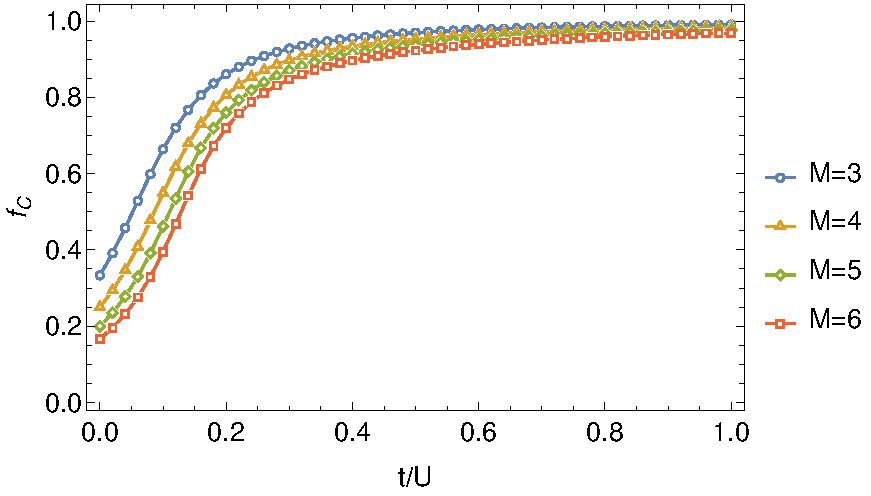
\includegraphics[height=5cm]{condensate_fraction_t_U} }}%
    \subfloat[\centering]{{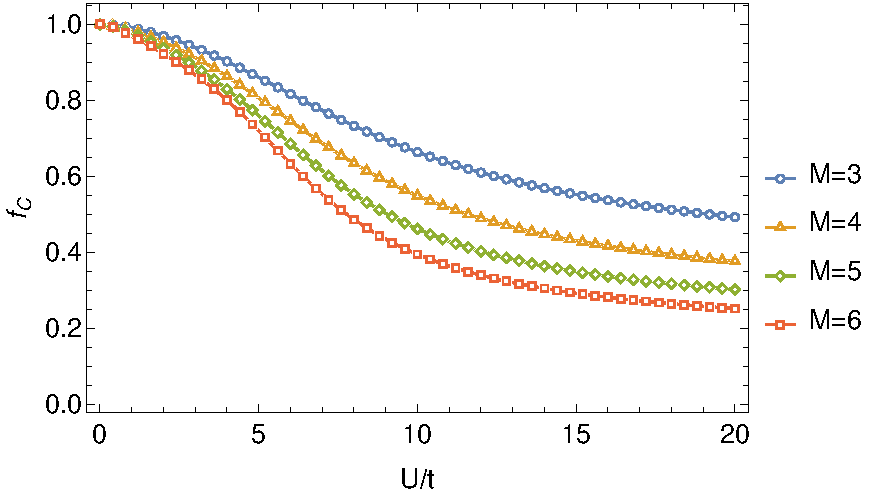
\includegraphics[height=4.9cm]{condensate_fraction_U_t} }}%
    \caption{Fracción de condensado $f_C=\lambda/N$, con $\lambda$
    el eigenvalor de la matriz de densidad reducida de una partícula.}%
    \label{fig:condensate_fraction}%
\end{figure}

\begin{figure}%
    \centering
    \subfloat[\centering]{{\includegraphics[height=5cm]{mu_t_u} }}%
    \subfloat[\centering]{{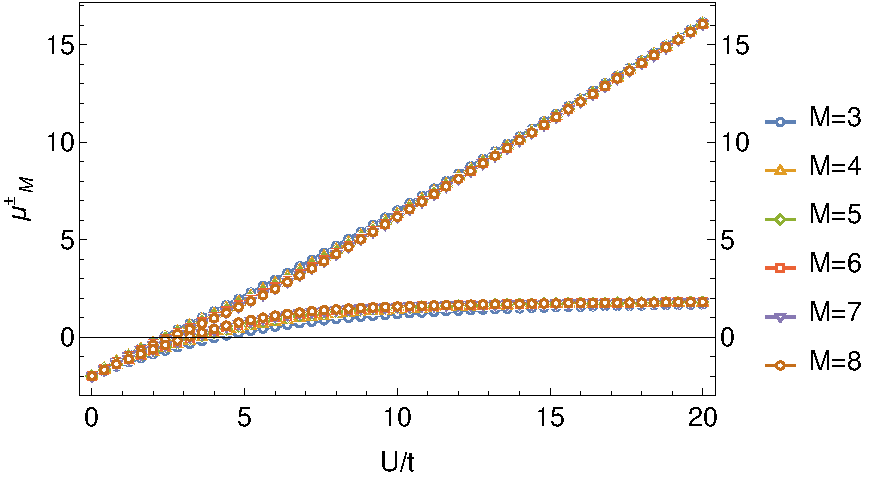
\includegraphics[height=4.9cm]{mu_U_t} }}%
    \caption{Potenciales químicos $\mu^{\pm}_M$.}%
    \label{fig:mus}%
\end{figure}

\begin{figure}%
    \centering
    \subfloat[\centering]{{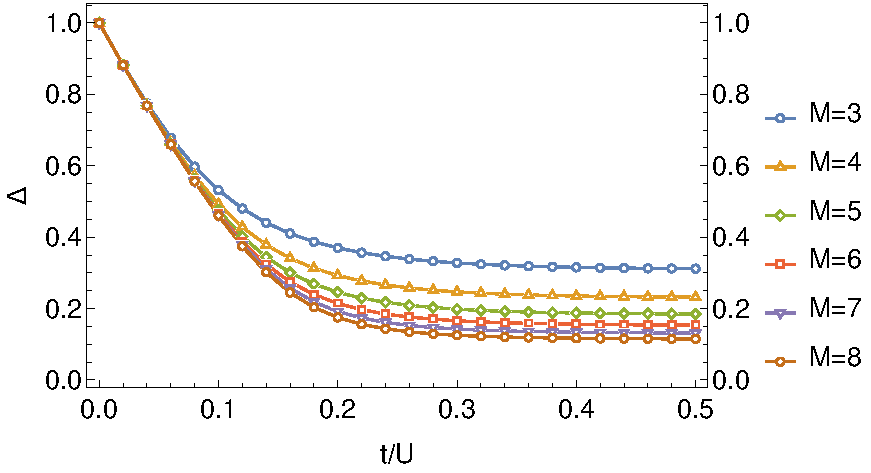
\includegraphics[height=5cm]{enery_gap_t_U} }}%
    \subfloat[\centering]{{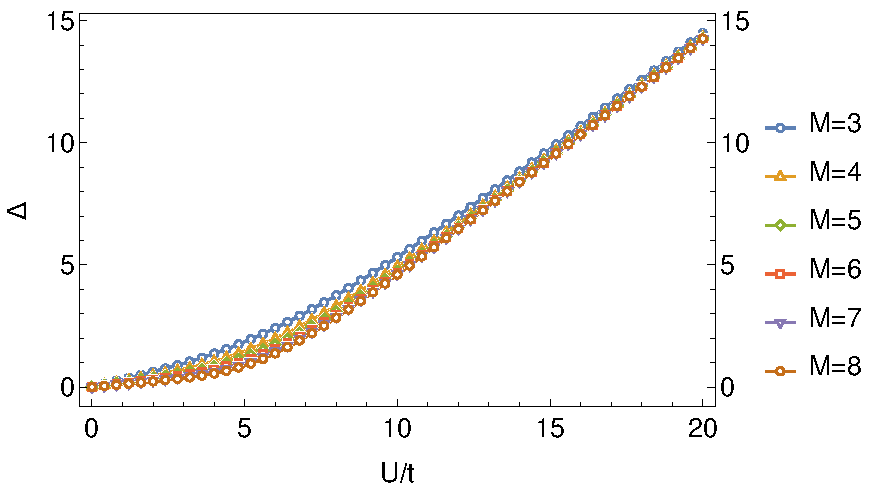
\includegraphics[height=4.9cm]{enery_gap_U_t} }}%
    \caption{Gap de enerǵía.}%
    \label{fig:gap}%
\end{figure}

\begin{figure}%
    \centering
    \subfloat[\centering]{{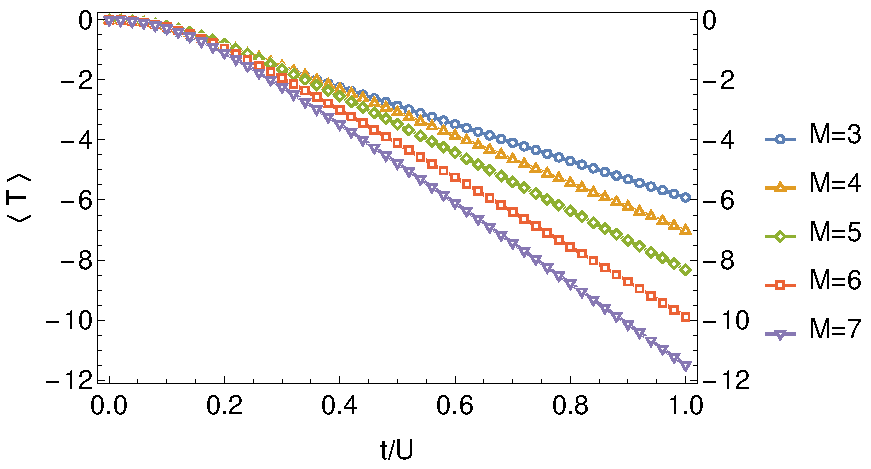
\includegraphics[height=5cm]{expVal_T_t_U} }}%
    \subfloat[\centering]{{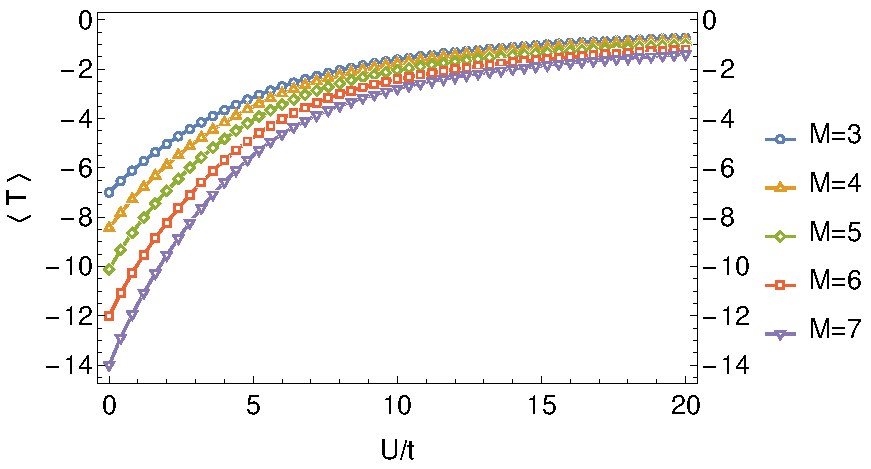
\includegraphics[height=4.9cm]{expVal_T_U_t} }}%
    \caption{Valor esperado de la energía cinética en el estado fundamental
    $\matrixel{G}{T}{G}$.}%
    \label{fig:expVal:T}%
\end{figure}

\begin{figure}%
    \centering
    \subfloat[\centering]{{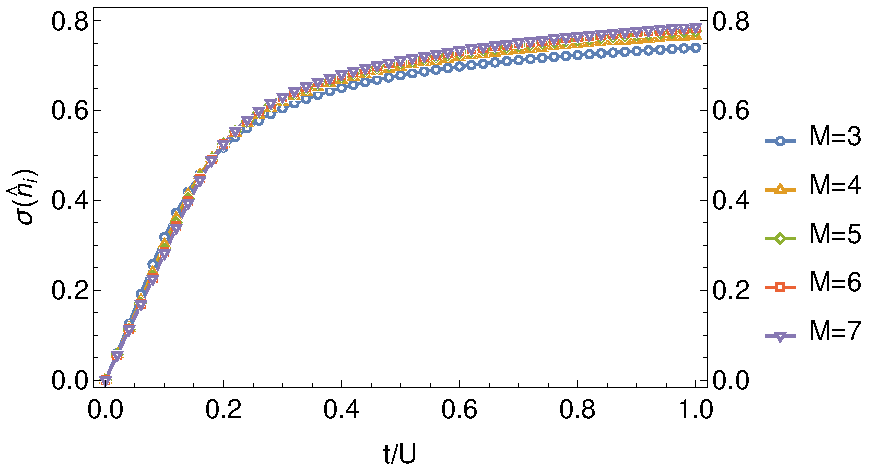
\includegraphics[height=5cm]{fluctuations_t_u} }}%
    \subfloat[\centering]{{\includegraphics[height=4.9cm]{fluctuations_u_t} }}%
    \caption{Fluctuaciones del operador de número $\hat n_i$.}%
    \label{fig:fluctuations}%
\end{figure}


\subsection{Discusión y conclusiones}
Debemos de recordar que el objetivo principal de este trabajo era didáctico, 
es decir, reproducir los resultados de algunos artículos tutoriales
\cite{zhang2010exact,raventos2017cold} que enseñan cómo realizar la diagonalización exacta del 
modelo de Bose-Hubbard y de otros artículos que estudiaron el modelo 
aplicado a algún sistema físico particular \cite{roth2003phase}. Este
objetivo princial se cumplió satisfactoriamente. Reprodujimos exitosamente
las gráficas de los potenciales químicos 
y el gap de energía en las Figs. 3 y 4 del artículo de Raventós, \textit{et. al.}
\cite{raventos2017cold} [Vea las Figs. 1.(a) y 2.(a) de este trabajo].
Así mismo, reprodujimos exitosamente los resultados de la Fig. 3 del 
artículo de \cite{zhang2010exact} para las fluctuaciones del número de
ocupación [Vea la Fig. 5.(a) de este trabajo]. También el comportamiento
de nuestras gráficas en las Figs. 5.(b), 2.(b) y 1.(b) coinciden 
cualitativamente con las gráficas de las Figs. 1, 2 y 3 del artículo 
de Roth y Burnett \cite{roth2003phase}.

Aunque no tenemos resultados con los que comparar nuestros resultados
de las gráficas en la Fig. 4 podemos decir que el comportamiento es 
el esperado, conforme el parámetro de \textit{hopping} se hace mayor
entonces la contribucción de la energía cinética debe aumentar (en 
valor absoluto). Por otro lado, en la Fig. 5.(b) notemos que conforme
aumenta el parámetro de la energía potencial entonces la contribución 
de la energía cinética tiende a cero. 

También se debe de mencionar que el ejercicio de la implementación numérica
puede hacerse más eficiente en el futuro, sin embargo, este trabajo fue un buen 
punto de partida y un ejercicio didáctico muy bueno para aprender cómo 
hacer diagonalización exacta y mejorar en el futuro el código.

En conclusión, se cumplió con el objetivo general de este trabajo, así 
como con los objetivos específicos. No obstante, debemos de mencionar que
la rutina para calcular la matriz de densidad de una partícula individual 
es ineficiente. En el futuro se deberá tener esto en cuenta y mejorar
la eficiencia del código.

\bibliographystyle{unsrt}
\bibliography{references}

\end{document}